\subsectionA{Tohr-Kreen}
Tohr-kreen are larger, cultured versions of thri-kreen. They are more civilized than their smaller cousins, and not nearly as aggressive. However, when they do fight, they are more deadly than the thri-kreen. They are occasionally met travelling about Athas, but none are native to the known lands. Rumors say that they may be from a city located far away, but no tohr-kreen will ever reveal the whereabouts of this city or if it even exists.

A tohr-kreen resembles its smaller cousin and may even be mistaken for one. They resemble a huge praying mantis with the sandy yellow coloring of a mantis warrior. They have dark purple or black eyes and wear a leather harness to carry weapons and other possessions. Tohr-kreen grow to as much as 3 meters high and 4 meters long and weigh from 150 to 200 kilograms. They carry normal weapons and shields, or the special weapon that the thri-kreen have developed, the gythka. They have also developed an improved version of the chatkcha, called a kyorkcha. A tohr-kreen encountered on the road usually has a specially made backpack, filled with art treasures and books it can't part with.

Tohr-kreen speak the language of the thri-kreen, and their own language as well.

% Zik-trin are a race bred by the zik-chil for loyalty and combat prowess. They are not a natural species, but rather are created from tohr-kreen or thri-kreen by the zik-chil in a deeply secretive and complicated ritual. Once the process is complete, the kreen is permanently changed into a zik-trin, and all memories of its former life are gone forever. Zik-trin faithfully serve the Priests of Change, the zik-chil, and obey only their orders. They are not automatons and are capable of thought and even speech (though they rarely choose to speak). It is simply that they are wholly loyal to their creators and live solely to serve them.
%
% Zik-trin measure several feet taller and longer than the average thri-kreen and weigh proportionately more.
%
% Zik-trin speak Thri-Kreen, on the rare occasions they choose to do so.

\subsubsection{Tohr-Kreen Society}
Tohr-kreen are known as zik-trin'ta by the kreen. They are covert scouts and secret operatives in service to the Tohr-Kreen Empire. They have been given a high degree of intellectual sophistication by their creators and display philosophical and pacifistic tendencies. This behavior is programmed by the Priests of Change, the zik-chil, who have sent the zik-trin'ta into the Tablelands to act as observers and spies. Often regarded with awe by other kreen, zik-trin'ta are seen as wise and noble philosophers by thri-kreen. This allows the zik-trin'ta to gather much information and exert influence in the interests of the Empire, all in preparation for the plans of their pale priests. Zik-trin'ta often amass lore and artifacts before returning to their homes in the Empire.

\begin{figure}[t!]
\centering
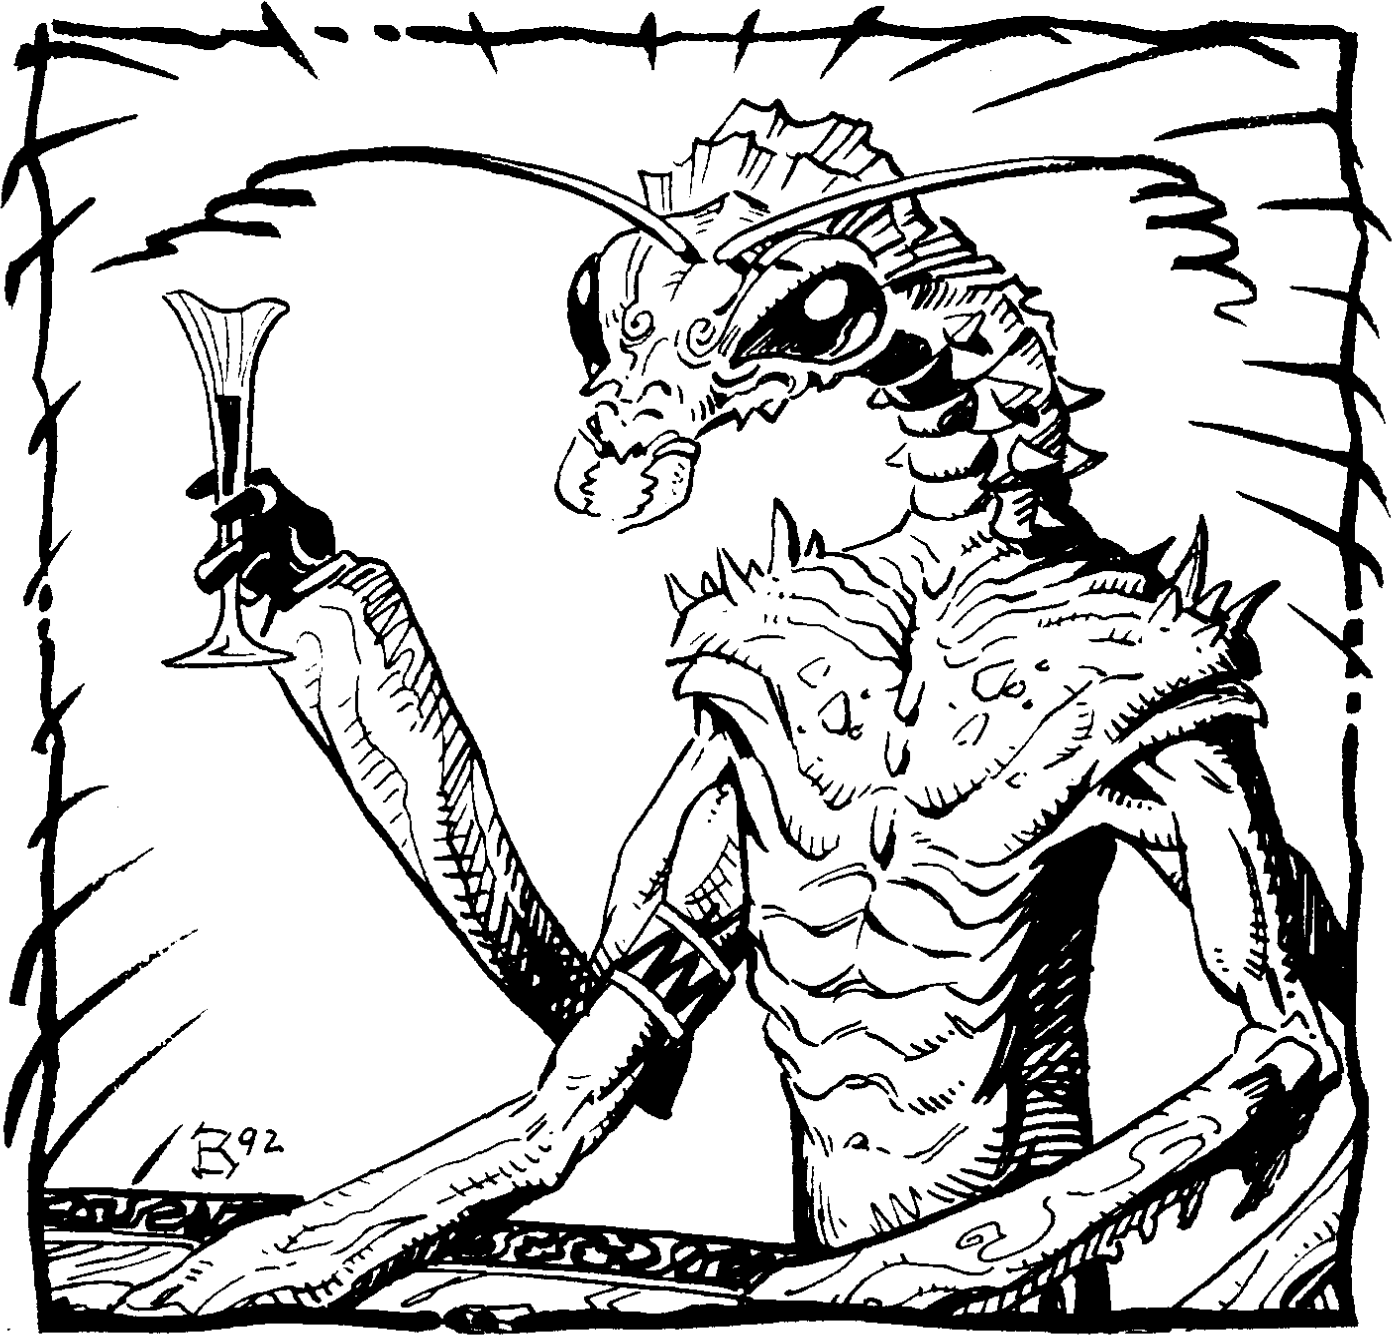
\includegraphics[width=\columnwidth]{images/tohrkreen-1.png}
\WOTC
\end{figure}

\subsubsection{Tohr-Kreen Racial Traits}
\begin{itemize*}
    \item +2 Strength, +2 Dexterity, +4 Constitution, +2 Intelligence, +2 Wisdom: tohr-kreen are more intelligent, relate easier to humanoids, and have higher endurance than their smaller cousins, but they are not as agile.
    \item Monstrous Humanoid: thri-kreen are not subject to spells or effects that affect humanoids only, such as \spell{charm person} or \spell{dominate person}.
    \item Large: As a Large creature, a tohr-kreen takes a $-1$ penalty to Armor Class, a $-1$ penalty on attack rolls, and a $-4$ penalty on \skill{Hide} checks. She gains a +4 size bonus on grapple checks, and her lifting and carrying limits are double those of Medium characters, but she uses bigger weapons than humans use.
    \item Tohr-kreen occupy a space of 3 meters and have a reach of 1.5 meters.
    \item Tohr-kreen base land speed is 33 meters.
    \item Darkvision: Tohr-kreen can see in the dark out to 18 meters. Darkvision is black and white only, but it is otherwise like normal sight, and half-giants can function just fine with no light at all.
    \item Racial Hit Dice: A tohr-kreen begins with 7 levels of monstrous humanoid, which provide 7d8 Hit Dice, a base attack bonus of +7, and base saving throw bonuses of Fort +2, Ref +5 and Will +5.
    \item Racial Skills: A tohr-kreen's monstrous humanoid levels give it skill points equal to 10 $\times$ (2 + Int modifier). Its class skills are \skill{Balance}, \skill{Climb}, \skill{Hide}, \skill{Jump}, \skill{Knowledge} (nature), \skill{Listen}, \skill{Spot}, and \skill{Survival}.
    \item A tohr-kreen's monstrous humanoid levels give it 3 feats.
    \item Sleep Immunity: Tohr-kreen do not sleep, and are immune to sleep spells and similar effects. Tohr-kreen spellcasters and manifesters still require 8 hours of rest before preparing spells or regaining power points.
    \item Natural Armor: Tohr-kreen have a +7 natural armor bonus to AC due to their naturally tough and resistant chitin.
    \item Multiple Limbs: Tohr-kreen have four arms, and thus can take the \feat{Multiweapon Fighting} feat instead of the \feat{Two-Weapon Fighting} feat. Tohr-kreen can also take the \feat{Multiattack} feat. (These are not bonus feats.)
    \item Natural Weapons: Tohr-kreen may make bite and claw attacks as a full round action. Their primary claw attack does 1d6 points of damage for each of their four claws. Their secondary bite attack, deals 1d4 points of damage, and has a chance to poison. A tohr-kreen can attack with a weapon (or multiple weapons) at its normal attack bonus, and make either a bite or claw attack as a secondary attack.
    \item Leap (Ex): Tohr-kreen are natural jumpers, gaining a +30 racial bonus to all \skill{Jump} checks.
    \item Deflect Arrows: Tohr-kreen gain the benefit of the \feat{Deflect Arrows} feat.
    \item Poison (Ex): A tohr-kreen delivers its poison with a successful bite attack. Fortitude DC 13 + Con modifier. The initial damage is paralysis for 2d6 rounds, and the secondary damage is 2d4 Con.
    \item Weapon Familiarity: To tohr-kreen, the chatkcha and gythka are treated as martial rather than exotic weapons. These weapons are more common among tohr-kreen than among other races.
    \item Tohr-kreen have no penalties wielding Medium-sized weapons.
    \item Tohr-kreen have a +4 racial bonus on \skill{Hide} checks in sandy or arid areas.
    \item Automatic Languages: Entomic, Kreen. Bonus Languages: Common, Dwarven, Elven, Saurian, and Terran.
    \item Favored Class: Bard.
    \item Level Adjustment: +3.
\end{itemize*}
